\documentclass[11pt]{article}
\usepackage[margin=1in]{geometry}
\usepackage{graphicx}
\usepackage{booktabs}
\usepackage{amsmath}
\usepackage{siunitx}
\usepackage[round]{natbib}
\usepackage[hidelinks]{hyperref}
\usepackage{caption}
\usepackage{placeins}
\captionsetup{font=small, labelfont=bf}

\title{Correcting AIFS Tropical Cyclone Intensity Forecasts:\\
a Scaled-Down Reproduction of AIFS-TC}
\author{Michel Faloughi\\ \small SCMP 5990 Independent Study, University of Pennsylvania}
\date{September 2026}

\begin{document}
\maketitle

\begin{abstract}
AI weather models such as ECMWF's AIFS-Single forecast tropical cyclone tracks well but
systematically underestimate intensity, because a $0.25^{\circ}$ grid cannot resolve the eyewall.
\citet{allen2026aifstc} showed that a simple machine-learned correction, trained on tabular features
of the forecast itself, removes most of this bias. This report reproduces the gradient-boosted half
of that work at reduced scale, using only public data: 399 operational AIFS-Single forecasts
covering every North Atlantic and East Pacific storm from February 2025 to September 2026, tracked
with a purpose-built MSLP-minimum tracker and corrected with gradient-boosted trees under
storm-grouped cross-validation. The raw model's maximum-wind mean absolute error (MAE) of
30.3\,kt is more than halved to 14.4\,kt, against 9.4\,kt for the official NHC forecast.
Raw-model error and the rapid-intensification failure mode match the paper almost exactly
(71.4\,kt vs.\ their 71.1\,kt raw MAE on RI cases), while the corrected error remains above the
paper's 11.0\,kt, consistent with training on one and a half seasons instead of nine years.
The tracker is validated against ECMWF's own operational AIFS tracks to within 1.1\,kt MAE.
\end{abstract}

\section{Introduction}

Data-driven weather models have reached operational skill for synoptic-scale prediction, and
ECMWF's AIFS-Single \citep{lang2024aifs} runs operationally alongside the physics-based IFS. For
tropical cyclones these models inherit a structural weakness: with grid spacing of about 28\,km,
the inner core of a hurricane is unresolved, so forecast 10\,m winds saturate far below observed
intensity even when the track is accurate. \citet{allen2026aifstc} (``AIFS-TC'') demonstrated that
this bias is largely \emph{predictable}: a gradient-boosted model over simple features of the AIFS
forecast and the operationally known initial intensity brings AIFS intensity forecasts to parity
with the operational frontier.

This project asks how much of that result survives a drastic reduction in resources: public data
only, one and a half hurricane seasons instead of nine years of hindcasts, a home-made tracker, and
a laptop. Beyond the replication itself, the by-product is an end-to-end open pipeline (catalog,
fetch, track, correct, evaluate) of roughly 900 lines of Python.

\section{Data}

\paragraph{AIFS forecasts.} The ECMWF Open Data AWS mirror (\texttt{s3://ecmwf-forecasts},
CC-BY-4.0) retains every operational AIFS-Single run since 2025-02-25. Storm lifetimes from the
IBTrACS best-track archive \citep{knapp2010ibtracs} define 399 forecast initializations (00/12
UTC) covering all North Atlantic (NA) and East Pacific (EP) storms of at least tropical-storm
strength through 2026-09-08. For each run, only the GRIB messages for mean sea-level pressure and
10\,m winds are downloaded via HTTP byte ranges, cropped to $0$--$60^{\circ}$N,
$180^{\circ}$W--$0^{\circ}$, at leads 0--168\,h every 6\,h (7.1\,GB total, versus hundreds of GB
for the full archive).

\paragraph{Reduction caveats.} The stored arrays are a lossy reduction: three surface variables,
one basin pair, leads capped at 168\,h (the mirror holds 360\,h), and winds stored in half
precision (error well below $0.1$\,kt, negligible against forecast error).

\paragraph{Operational archive, not hindcasts.} Unlike the paper's controlled hindcast training
set, these are the forecasts actually issued in real time. Two consequences matter. First, the
model version changes mid-dataset: AIFS-Single 1.0 was operational for the 2025 season and 2.0
(released 2026-05-12) for 2026; a version flag is passed to the correction model and results are
reported by season. Second, each run starts from the real-time operational analysis with its
data-assimilation cutoff, not from a reanalysis.

\paragraph{Verification and benchmarks.} Ground truth is the IBTrACS/ATCF best track (USA agency
values). The benchmark is OFCL, the official human forecast of the National Hurricane Center,
parsed from the ATCF a-deck archive, which also supplies GDMN, the ensemble mean of Google
DeepMind's cyclone model \citep{deepmind2025weatherlab}, and EAIO, ECMWF's own tracker applied to
the same AIFS runs.

\section{Methods}

\paragraph{Tracker.} Each forecast is seeded at the best-track position at initialization. At each
6\,h step the storm is located at the MSLP minimum within 450\,km of a first guess (previous
position advected with previous motion) on a lightly smoothed field; intensity is that minimum
pressure and the maximum 10\,m wind within 250\,km. Tracking stops when the low is no longer
distinct. Against ECMWF's operational AIFS tracks (EAIO) at matched initialization and lead
($n=1209$, 24 storms), the tracker agrees to a mean difference of $+0.8$\,kt and an MAE of
1.1\,kt, so tracker choice is not a meaningful error source.

\paragraph{Correction model.} Following the GBM branch of AIFS-TC, gradient-boosted trees
(scikit-learn \texttt{HistGradientBoostingRegressor}, 5-seed average) predict the residual between
best-track and AIFS maximum wind. The 22 features include the AIFS forecast state and its trends
and running extremes, translation speed, basin, day of year, the model-version flag, storm age,
the observed intensity and 12/24\,h intensity trend at initialization, and the initial AIFS bias.
Observed rapid-intensification cases (RI, $\ge 30$\,kt observed gain in 24\,h) are weighted
$2\times$ in training, as in the paper. Evaluation uses storm-grouped 5-fold cross-validation, so
a storm is never corrected by a model that saw any part of it. A persistence-of-initial-bias
baseline (carrying the initialization-time AIFS bias forward unchanged) is included as a sanity
check; the GBM beats it at every lead beyond 24\,h.

\section{Results}

Table~\ref{tab:main} and Figure~\ref{fig:mae} give the headline result on the homogeneous sample
(cases where raw, corrected, and OFCL forecasts all exist and verify against best track):
the correction cuts overall MAE from 30.3 to 14.4\,kt, with non-overlapping 95\% confidence
intervals from a storm-level bootstrap. It does not reach OFCL (9.4\,kt) overall, but approaches
it at long leads (16.4 vs.\ 14.1\,kt at 120\,h). On a separate homogeneous sample containing
GDMN ($n=2022$, 41 storms), DeepMind's dedicated cyclone model scores 9.9\,kt, on par with OFCL
(9.6), with corrected AIFS at 14.6.

\begin{table}[t]
\centering
\caption{Maximum-wind MAE (kt) versus best track by forecast lead time, homogeneous sample
($n=2223$ cases, 46 storms, NA+EP, Feb 2025--Sep 2026). Bottom row: all leads pooled, with 95\%
storm-bootstrap confidence intervals.}
\label{tab:main}
\begin{tabular}{rrccc}
\toprule
Lead (h) & $n$ & AIFS raw & AIFS+GBM & NHC OFCL \\
\midrule
 12 & 442 & 26.4 & 10.8 &  4.9 \\
 24 & 396 & 28.4 & 13.2 &  7.4 \\
 36 & 358 & 29.8 & 14.9 &  9.5 \\
 48 & 315 & 31.4 & 16.3 & 10.9 \\
 72 & 247 & 33.4 & 16.6 & 11.5 \\
 96 & 190 & 35.2 & 16.7 & 12.8 \\
120 & 148 & 35.8 & 16.4 & 14.1 \\
144 &  74 & 31.7 & 16.3 & 13.6 \\
168 &  53 & 25.0 & 14.2 & 11.1 \\
\midrule
12--168 & 2223 & 30.3 [24.5, 35.1] & 14.4 [12.4, 16.6] & 9.4 [8.0, 10.5] \\
\bottomrule
\end{tabular}
\end{table}

\begin{figure}[t]
\centering
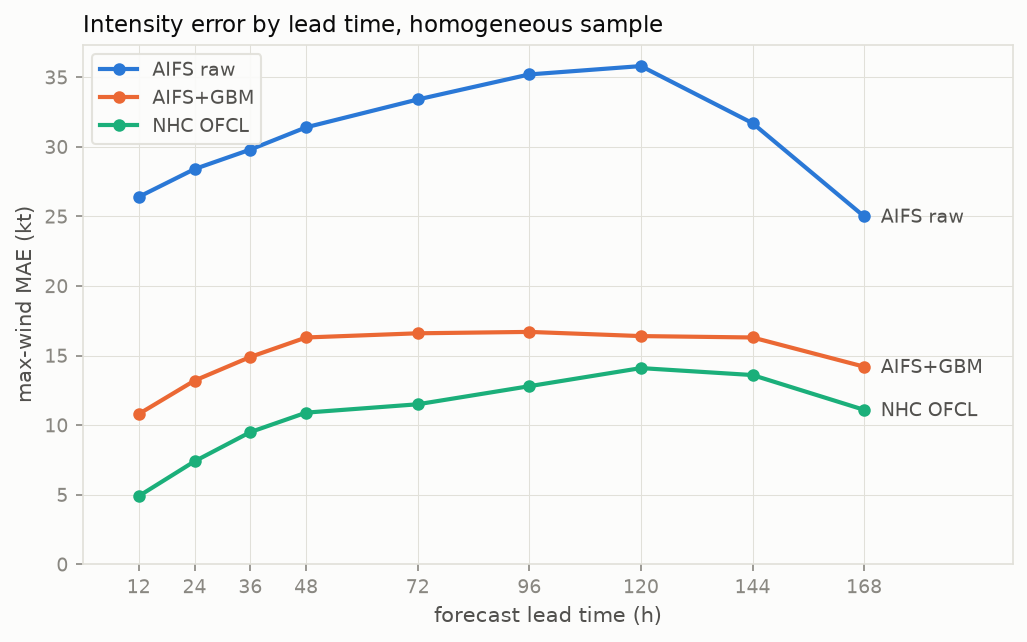
\includegraphics[width=0.85\linewidth]{figures/tc_mae_by_lead.png}
\caption{Maximum-wind MAE by lead time on the homogeneous sample. The raw AIFS error is
dominated by the under-resolution bias; the GBM correction removes most of it at every lead.}
\label{fig:mae}
\end{figure}

Table~\ref{tab:subsets} breaks the pooled result down. The correction helps in both basins and
both seasons. Notably, it performs better on the 2026 season (AIFS-Single 2.0, 12.1\,kt) than on
2025 (v1.0, 15.5\,kt) despite 2026 contributing less training data, suggesting the newer model's
errors are more systematic and therefore easier to learn. Rapid intensification remains the hard
case: raw AIFS misses RI by 71.4\,kt on average, the correction recovers roughly half of that
(38.3\,kt), and the human forecast (20.2\,kt) stays well ahead.

\begin{table}[t]
\centering
\caption{Pooled (12--168\,h) maximum-wind MAE (kt) with 95\% storm-bootstrap confidence
intervals, by subset.}
\label{tab:subsets}
\begin{tabular}{lrrccc}
\toprule
Subset & $n$ & Storms & AIFS raw & AIFS+GBM & NHC OFCL \\
\midrule
All cases          & 2223 & 46 & 30.3 [24.5, 35.1] & 14.4 [12.4, 16.6] &  9.4 [8.0, 10.5] \\
RI cases only      &  162 & 13 & 71.4 [61.7, 77.5] & 38.3 [32.0, 42.8] & 20.2 [16.5, 23.5] \\
North Atlantic     &  772 & 15 & 32.4 [22.0, 39.3] & 15.5 [10.7, 19.7] & 10.4 [7.7, 12.4] \\
East Pacific       & 1451 & 31 & 29.2 [22.2, 35.7] & 13.9 [11.4, 16.2] &  8.9 [7.4, 10.2] \\
2025 (AIFS 1.0)    & 1526 & 30 & 29.6 [23.2, 35.5] & 15.5 [12.9, 18.1] &  9.6 [8.2, 10.9] \\
2026 (AIFS 2.0)    &  697 & 16 & 31.8 [20.1, 39.2] & 12.1 [8.4, 14.5]  &  8.8 [5.8, 10.9] \\
\bottomrule
\end{tabular}
\end{table}

Figure~\ref{fig:lowell} shows the raw bias at its most dramatic: Hurricane Lowell (EP, 2026)
reached 140\,kt while every raw AIFS forecast saturated near 60\,kt. Figure~\ref{fig:map} shows
the underlying fields and tracks for one initialization with three simultaneous storms.

\begin{figure}[t]
\centering
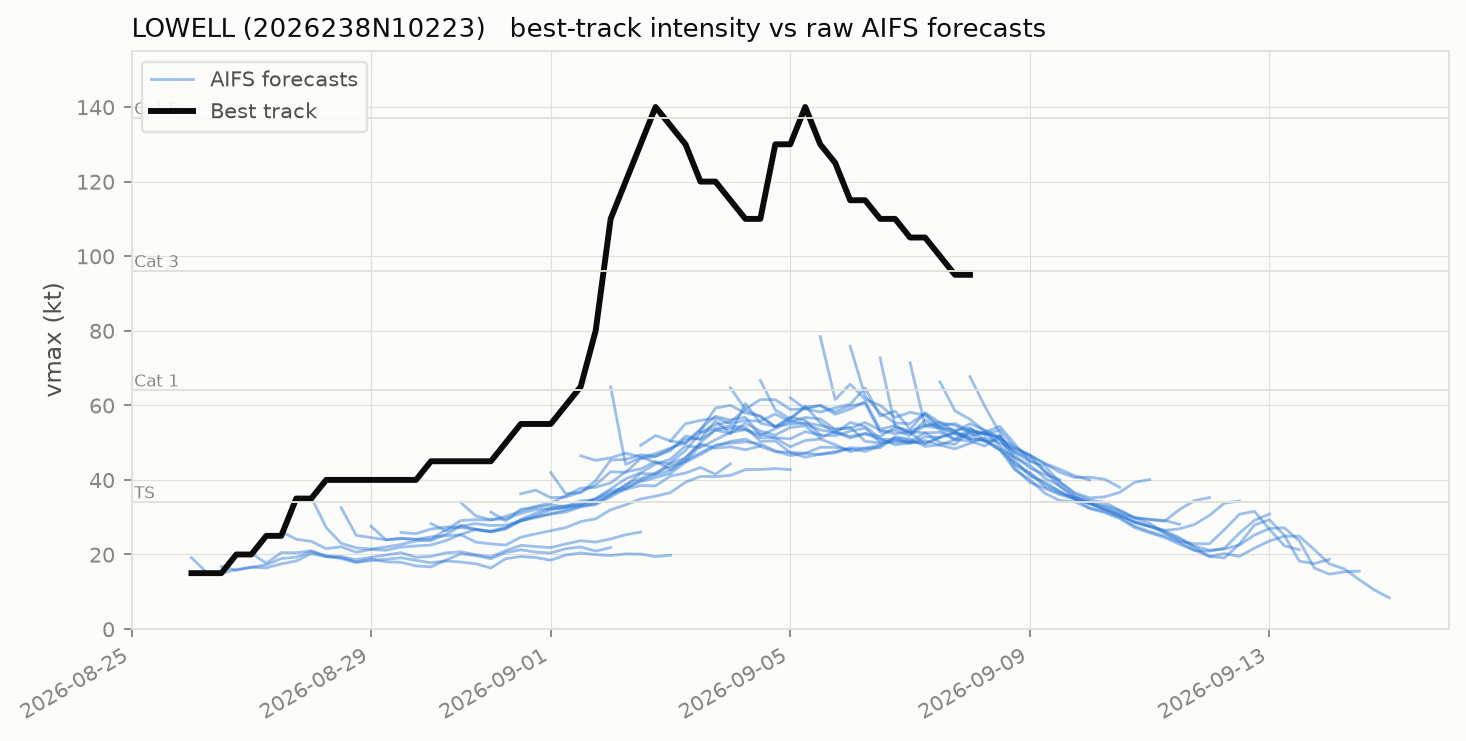
\includegraphics[width=0.9\linewidth]{figures/tc_intensity_lowell.png}
\caption{Observed intensity of Hurricane Lowell (2026, EP; black) against all 27 raw AIFS
forecasts (blue). The model's track is good but its intensity saturates near 60\,kt against an
observed peak of 140\,kt: the under-resolution bias the correction targets.}
\label{fig:lowell}
\end{figure}

\begin{figure}[t]
\centering
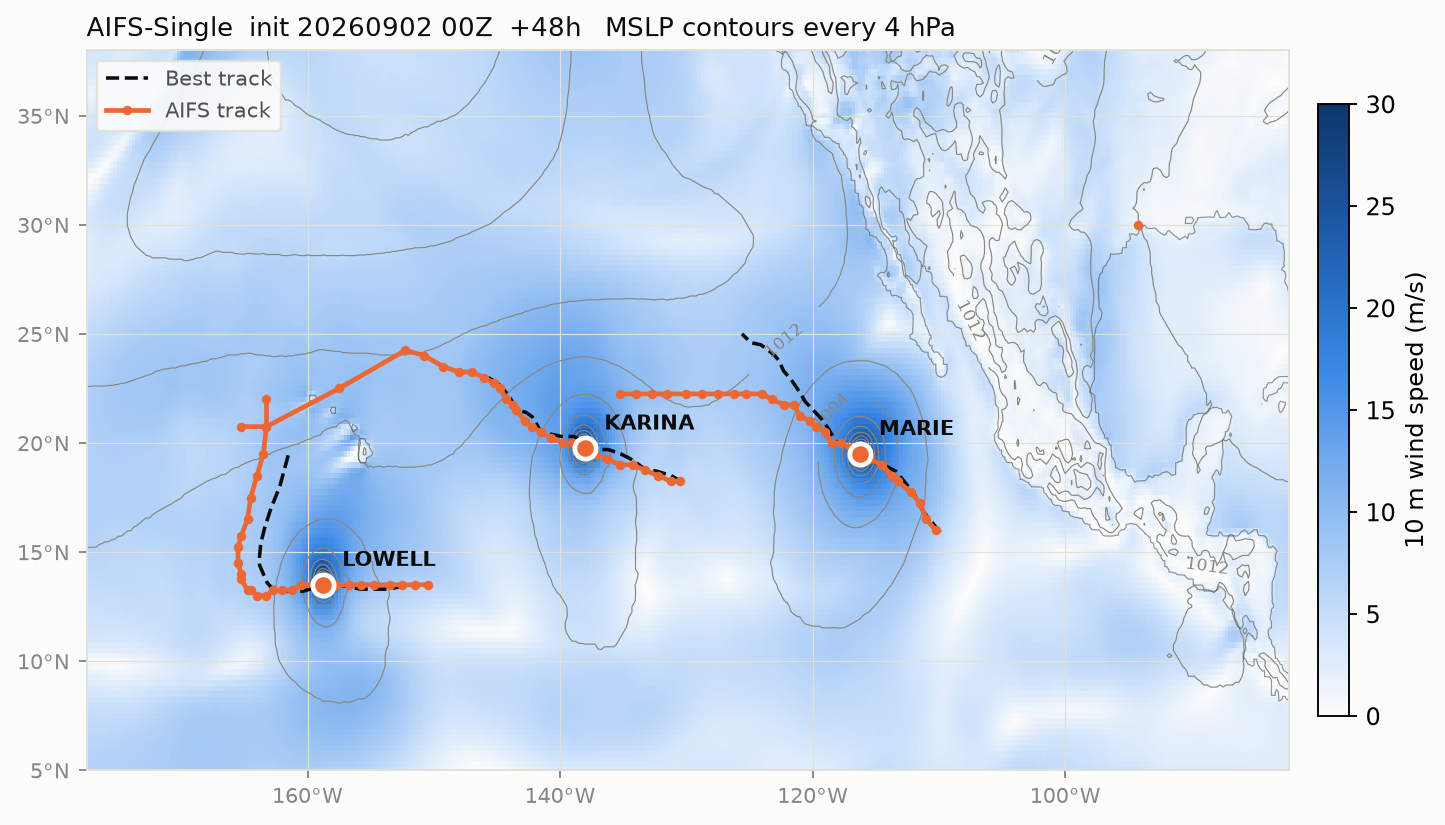
\includegraphics[width=0.95\linewidth]{figures/tc_map_2026090200_048h.png}
\caption{AIFS-Single forecast fields at $+48$\,h from the 2026-09-02 00Z run: 10\,m wind speed
(shading), MSLP (contours every 4\,hPa), forecast tracks (orange) and best tracks (dashed) for
hurricanes Lowell, Karina and Marie.}
\label{fig:map}
\end{figure}

\section{Comparison with AIFS-TC}

Table~\ref{tab:paper} sets these results against the paper's NA+EP evaluation
\citep{allen2026aifstc}. The samples differ (their held-out 2025 under one model version and
hindcast initial conditions; here 2025--2026 operational output under two versions), so each
column should be read against its own OFCL, not across columns.

\begin{table}[t]
\centering
\caption{Pooled maximum-wind MAE (kt), this work versus AIFS-TC (their NA+EP test set, 29
storms). Samples differ; compare each system to its own sample's OFCL.}
\label{tab:paper}
\begin{tabular}{lcc}
\toprule
 & This work & AIFS-TC \\
\midrule
AIFS raw            & 30.3 & 35.3 \\
Corrected           & 14.4 & 11.0 \\
NHC OFCL            &  9.4 & 10.7 \\
AIFS raw, RI only   & 71.4 & 71.1 \\
Corrected, RI only  & 38.3 & 20.9 \\
OFCL, RI only       & 20.2 & 20.1 \\
\bottomrule
\end{tabular}
\end{table}

Three observations. First, the \emph{baselines} land on the paper's numbers: raw AIFS error is
the same phenomenon at the same magnitude, and on RI cases the agreement is striking (71.4 vs.\
71.1\,kt). Together with the 1.1\,kt tracker agreement, this indicates the pipeline measures the
same quantity the paper measures. Second, the \emph{correction} reproduces the qualitative claim,
recovering roughly three quarters of the raw-to-OFCL gap, but not the paper's parity with OFCL.
Third, the shortfall concentrates exactly where limited training data should hurt most: rare RI
events, of which this dataset contains 13 storms' worth against the paper's nine years. The
2026-only result (12.1\,kt, single model version) already approaches the paper's 11.0.

\section{Limitations}

One and a half seasons versus nine years of training data; two model versions in one dataset,
handled only by a feature flag; the GBM branch only (no CNN over three-dimensional patches);
best-track initial intensity as a feature where fully operational practice would use the
real-time CARQ estimate (the paper reports both variants); two basins; leads capped at 168\,h.
Position errors are measured but not corrected.

\FloatBarrier
\section{Reproducibility}

All code is at \url{https://github.com/MichelFaloughi/scmp-5990} (directory \texttt{pipeline/}). The
7.1\,GB of forecast data regenerates from public sources with two commands (catalog and fetch);
the full pipeline runs on a laptop in minutes thereafter. Data sources: ECMWF Open Data
(CC-BY-4.0), IBTrACS v04r01, and the NHC ATCF archive.

\bibliographystyle{plainnat}
\bibliography{refs}

\end{document}
